\begin{figure}[t!]
\begin{center}
\centerline{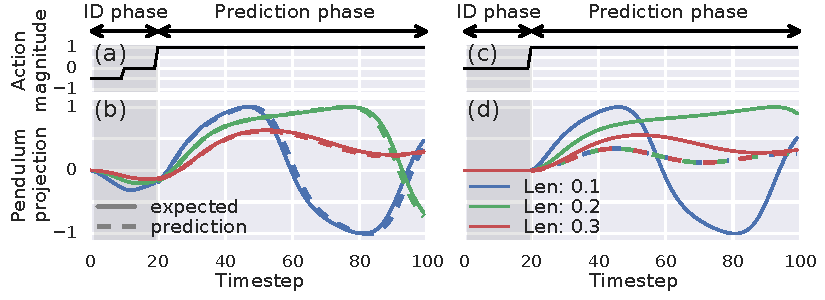
\includegraphics[width=\columnwidth]{figures/sysid_pendulum}}
\vspace{-0.1in}
\caption{System identification analysis in Pendulum. (a) Control inputs are applied to three Pendulums with different, unobservable lengths during the 20-step ID phase, which makes the system identifiable. (b) The model's predicted trajectories (dashed curves) track the ground truth (solid curves) closely in the subsequent 80-step prediction phase. (c) No control inputs are applied to the same systems during the ID phase, which makes the system identifiable. (d) The model's predicted trajectories across systems are very different from the ground truth.
}
\label{fig:sysid_pendulum}
\end{center}
\vskip -0.35in
\end{figure}